\documentclass[11pt]{article}

\newcommand{\numpy}{{\tt numpy}}    % tt font for numpy

\usepackage{graphicx}
\usepackage{listings}

\topmargin -.75in
\textheight 9in
\oddsidemargin -.25in
\evensidemargin -.25in
\textwidth 7in

\begin{document}

$$\mbox{\Large \bf CS 111: Homework 2: Due by 11:59pm Monday, January 20}$$

\medskip\noindent
{\bf Submit your homework online as a PDF file to GradeScope,
and tell GradeScope which page(s) contain each problem.}

\par\bigskip
{\bf 1.}
Consider the code for the temperature problem in 
the lecture file {\tt temperature.py}, 
especially the routines {\tt make\_A()} and {\tt make\_b()}
that create the matrix $A$ and right-hand side $b$.
Experiment with different ways of setting the boundary conditions,
which are the parameters {\tt top}, {\tt bottom}, {\tt left}, and {\tt right} 
to {\tt make\_b()}.
Make a plot of the most interesting result that you get (in your opinion), 
and explain how you got it. 
If you want, you can also experiment with {\tt matplotlib} 
to make a more interesting plot of your result. 
(The CS 111 logo on the course web page was obtained this way in 2010; 
maybe we can get a new logo this year!)

\par\bigskip
{\bf 2.}
Again consider the routines {\tt make\_A()} and {\tt make\_b()}
that create the matrix~$A$ and right-hand side~$b$ for the temperature problem.
Let $k=100$.

\par\medskip
{\bf 2a.}
How many elements are there in $b$?

\par\medskip
{\bf 2b.}
Considering all possible choices for the temperatures on the boundary,
what is the largest number of elements of $b$ that could possibly 
be nonzero? 

\par\medskip
{\bf 2c.}
Explain why the rest of the elements of $b$ are zero, no matter
what the boundary temperatures are.

\par\bigskip
{\bf 3.}
Write the following matrix in the form $A=LU$, 
where $L$ is a unit lower triangular matrix
(that is, a lower triangular matrix with ones on the diagonal) 
and $U$ is an upper triangular matrix.
$$A =
   \left(
   \begin{array}{ccc}
    4 & -1 & -1 \\ 	
   -1 &  4 & -1 \\ 
   -1 & -1 &  4 \\
   \end{array} \right)
$$

\par\bigskip
{\bf 4.}
The following three statements are all {\bf false}. For each one, 
give a counterexample consisting of a 3-by-3 matrix or matrices, 
and show the computation that proves that the statement fails.

\par\medskip
{\bf 4a.}
If $P$ is a permutation matrix and $A$ is any matrix, then $PA=AP$.

\par\medskip
{\bf 4b.}
If matrix $A$ is nonsingular, then it has a factorization $A=LU$
where $L$ is lower triangular and $U$ is upper triangular.

\par\medskip
{\bf 4c.}
The product of two symmetric matrices is a symmetric matrix.

\newpage
\par\bigskip
{\bf 5a.} Consider the permutation matrix 
$$P =
   \left(
   \begin{array}{cccc}
    0 & 1 & 0 & 0 \\ 	
    0 & 0 & 0 & 1 \\ 	
    0 & 0 & 1 & 0 \\ 	
    1 & 0 & 0 & 0 \\ 	
   \end{array} \right)
$$
Find a 4-element permutation vector {\tt v = np.array(something)}
such that, for {\em every}\, 4-by-4 matrix $A$, 
we have {\tt A[v,:] == P @ A}.
Test your answer by running a few lines of Python, 
and turn in the result.

\par\medskip
{\bf 5b.} For the same $P$, 
find a 4-element permutation vector {\tt w = np.array(something)}
such that, for {\em every}\, 4-by-4 matrix $A$, 
we have {\tt A[:,w] == A @ P}. 
Test your answer and turn in the result.

\par\bigskip
{\bf 6.}
Write {\tt Usolve()}, analogous to {\tt Lsolve()} in 
the lecture file {\tt LU.py},
to solve an upper triangular system $Ux=y$. 
Warning: Notice that, unlike in {\tt Lsolve()}, 
the diagonal elements of $U$ don't have to be equal to one.
Test your answer, both by itself and with {\tt LUsolve()},
and turn in the result.
Hint: Loops can be run backward in Python, 
say from $n-1$ down to $0$, by writing
$$\mbox{\tt for i in reversed(range(n)):}$$

\newpage
\begin{enumerate}

\item 
The graph is obtained by setting the quarter portion of the end of each side to 100 degree and the midpoint of each side to 500 degree. The graph is plotted with a cyclic color mapping, which is why some of the hottest points of the map is black like they are cold. \newline
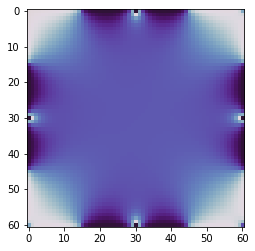
\includegraphics{index}

\item 
{\bf a.} 10,000\\
{\bf b.} 396\\
{\bf c.} Because the equation dictates that the right hand side is zero as the sum of the pixel and the negative average of the pixels around it should be equal

\item
$$U =
\left(
\begin{array}{ccc}
4 & -1 & -1 \\ 	
0 & \frac{15}{4} & -\frac{5}{4} \\ 
0 & 0 &  \frac{10}{3} \\
\end{array} \right)
$$
$$L =
\left(
\begin{array}{ccc}
1 & 0 & 0 \\ 	
-\frac{1}{4} & 1 & 0 \\ 
-\frac{1}{4} & -\frac{1}{3} & 1 \\
\end{array} \right)
$$

\item 
{\bf a.} $$P =
\left(
\begin{array}{ccc}
0 & 0 & 1\\ 
0 & 1 & 0\\
1 & 0 & 0
\end{array} \right), A = 
\left(
\begin{array}{ccc}
1 & 2 & 3\\
4 & 5 & 6\\
7 & 8 & 9
\end{array} \right)
$$
$$
PA = 
\left(
\begin{array}{ccc}
7&8&9\\
4 & 5 & 6\\
1&2&3
\end{array} \right) \neq
AP = \left( \begin{array}{ccc}
3&2&1\\
6&5&4\\
9&8&7
\end{array} \right)
$$\\
{\bf b.} 
$$
A = \left(
\begin{array}{ccc}
	0 & 1 & 1\\ 	
	1 & 1 & 0\\
	1 & 2 & 0
\end{array} \right)
$$
{\bf c.}
$$
\left(
\begin{array}{ccc}
1 & 2 & 7\\
2 & 5 & 6\\
7 & 6 & 9
\end{array} \right) \cdot
\left(
\begin{array}{ccc}
0 & 0 & 1\\
0 & 1 & 0\\
1 & 0 & 0
\end{array} \right) = 
\left(
\begin{array}{ccc}
7 & 2 & 1\\
6 & 5 & 2\\
9 & 6 & 7
\end{array} \right)
$$

\item 
{\bf a.}
$$
\left(
\begin{array}{cccc}
	1 & 3 & 2 & 0
\end{array} \right)
$$
{\bf b.}
$$
\left(
\begin{array}{cccc}
3 & 0 & 2 & 1
\end{array} \right)
$$

\item 
\lstset{language=Python}
\lstset{frame=lines}
\lstset{caption={Usolve}}
\lstset{label={lst:code_direct}}
\lstset{basicstyle=\footnotesize}
\begin{lstlisting}
def Usolve(U, b):
"""Backward solve a unit upper triangular system Uy = b for y
Parameters: 
U: the matrix, must be square, upper triangular
b: the right-hand side vector
Output:
y: the solution vector to U @ y == b
"""

# Check the input
m, n = U.shape
assert m == n, "matrix U must be square"
assert np.all(np.triu(U) == U), "matrix U must be upper triangular"

# Make a copy of b that we will transform into the solution
y = b.astype(np.float64).copy()

# Backwards solve
for col in reversed(range(n)):
y[col] = y[col] / U[col, col]
y[0:col] -= y[col] * U[0:col:, col]

return y
\end{lstlisting}
\end{enumerate}

\end{document}
